\chapter{Đánh giá thực nghiệm tái lập}
\label{chap:experiments}

\section{Câu hỏi thực nghiệm và thiết kế đối chiếu}

Năm giả thuyết được đánh giá: H1 tổng tiền tố giảm chi phí truy hồi forest; H2 danh sách thưa có lợi khi ít nhãn thật; H3 quét sự kiện thay thế ma trận TTSP với ít phép toán và bộ nhớ; H4 compact terminal, pruning, join index và giải phóng bảng có tác dụng đo được; H5 các solver đúng theo cả hai ngữ nghĩa và vẫn xử lý được trường hợp có số tuyến hàm mũ.

Baseline \code{forest-paper} là bản cài lại truy hồi công bố của Enright và cộng sự, sau cùng phép nén hạng và dùng cùng kiểu BigInt. Nó không phải mã tác giả. \code{ttsp-transfer} và \code{tw-dp-baseline} là các phiên bản trước trong repository. Vì bài báo gốc không có artifact thực nghiệm MSO, không báo speedup so với một chương trình MSO chưa được cài đặt. \code{brute} là đối chiếu enumeration trên cùng input; trên graph nhỏ nó có thể nhanh hơn DP.

\section{Môi trường và phương pháp đo}

Máy đo dùng Intel Core i9-9980HK, RAM khoảng 15 GiB, Linux 6.12.93 x86-64, GCC 14.3.0, Python 3.13.12; cờ biên dịch \code{-std=c++20 -O3 -DNDEBUG}. Tiến trình điều phối và con được pin vào CPU đầu tiên được phép, trong lần đo này là CPU 0. Không khóa DVFS và không khẳng định toàn bộ máy không có hoạt động nền.

Mỗi solver/cell hoàn thành có một lượt calibration/warm-up và bảy subprocess batch ghi nhận. Với lời gọi rất ngắn, số lặp nội bộ được chọn để nhắm khoảng 10 ms, tối đa 256 lần. Mỗi lần xây trạng thái solver mới; TG chỉ đọc một lần trong batch. Thứ tự solver ở mỗi replicate được xáo bằng seed xác định. Median và IQR được tính theo bảy giá trị per-call; error bar từ Q1 đến Q3, không phải khoảng tin cậy 95\%.

Timed region gồm solver và đọc/validate decomposition, nhưng loại đọc/nén TG và sinh decomposition. CSV lưu riêng parse time và thời gian toàn subprocess batch; chúng không bị nhầm với thời gian một query độc lập. Khi parsing chi phối, speedup end-to-end sẽ thấp hơn speedup solver. CPU time lấy từ đồng hồ CPU của tiến trình C++, không từ Python điều phối.

Trên Linux, peak RSS lấy từ \code{VmHWM} trong \code{/proc/self/status} của address space sau exec. Một đợt đo trước dùng \code{ru\_maxrss} đã được phát hiện có thể giữ đỉnh RSS của Python trước exec; toàn bộ bảng cuối được đo lại sau khi sửa và dữ liệu cũ lưu riêng. RSS vẫn bao gồm parser và allocator retention, nên khác peak số trạng thái đang sống. Giới hạn virtual address space là 1536 MiB; timeout là ba giây cho \emph{toàn subprocess}, không chỉ vùng solver. Ma trận có compressed $r>128$ bị skip theo ngân sách định trước.

\section{Bộ dữ liệu và đơn vị báo cáo}

Chiến dịch chính có 169 cấu hình: 49 forest dày, 9 forest thưa, 5 density control, 45 diamond all-times, 7 diamond mở rộng/strict, 3 diamond thưa lớn, 24 partial 2-tree, 12 width sensitivity, 4 enumeration crossover, 3 ablation và 8 cactus. Bổ sung 21 ladder cho tổng \BenchCases{} cấu hình. Có \BenchSuccessfulSamples{} mẫu thành công, \BenchTimeouts{} bản ghi timeout và \BenchSkips{} skip ngân sách. Mọi raw record được giữ trong CSV.

Master seed $20260928$ được băm cùng family, cell và replicate. RNG duyệt cạnh theo thứ tự canonical, tránh phụ thuộc thứ tự set. Partial $k$-tree sinh cùng decomposition đã biết; bộ Graph Atlas dùng degree-two elimination để nhận dạng đúng lớp width không quá hai. Hash input, decomposition, source, executable và script điều phối được lưu để ngăn dùng nhầm phiên bản.

Các số lượng cần phân biệt: một graph có nhiều truy vấn; một truy vấn có hai ngữ nghĩa; một lượt query/ngữ nghĩa có nhiều đối chiếu solver; một cell hiệu năng có bảy mẫu. Không gọi tất cả chúng là ``số instance độc lập''. Các chiến dịch có thể chồng lặp cấu hình, nên tổng lượt audit không phải số graph phân biệt.

\section{Kiểm chứng tính đúng}

\begin{table}[htbp]
\centering
\small
\setlength{\tabcolsep}{4pt}
\caption{Kiểm chứng mới; mỗi cặp đầu cuối được thử theo cả hai ngữ nghĩa thời gian.}
\label{tab:audit-expanded}
\begin{tabular}{lrrr}
\toprule
Chiến dịch & \shortstack{Truy vấn/\\ngữ nghĩa} & \shortstack{Đối chiếu\\solver} & Sai lệch \\
\midrule
Vét cạn $n=2,r=2$ & 16 & 64 & 0 \\
Vét cạn $n=3,r=2$ & 768 & 3\,072 & 0 \\
Vét cạn $n=4,r=2$ & 98\,304 & 340\,728 & 0 \\
Vét cạn $n=5,r=1$ & 40\,960 & 147\,800 & 0 \\
Rừng ngẫu nhiên & 2\,000 & 10\,000 & 0 \\
TTSP ngẫu nhiên & 2\,000 & 6\,000 & 0 \\
Partial $k$-tree, $k=1..4$ & 2\,000 & 6\,000 & 0 \\
Cactus ngẫu nhiên & 2\,000 & 4\,000 & 0 \\
Đổi đỉnh và nhãn thời gian & 400 & 800 & 0 \\
Graph Atlas, width $\le2$ & 111\,408 & 222\,816 & 0 \\
\textbf{Tổng lượt} & 259\,856 & 741\,280 & 0 \\
\bottomrule
\end{tabular}
\end{table}


Vét cạn $n\le4,r=2$ gán cho mỗi cặp đỉnh một trong bốn trạng thái: vắng, chỉ thời điểm 1, chỉ thời điểm 2, hoặc cả hai. Mọi cặp terminal có thứ tự và cả hai ngữ nghĩa được xét. Thử thêm toàn bộ graph năm đỉnh tại một thời điểm; tập này bao gồm graph width lớn hơn hai. Oracle C++ liệt kê trực tiếp time-edge sequences; bản DP tối ưu và baseline cùng được so khớp.

Graph Atlas phân phối 1253 graph không đẳng cấu có tối đa bảy đỉnh \cite{atlas1998}. Có \AtlasGraphs{} graph với ít nhất hai đỉnh và width không quá hai được chọn, gồm cả graph không liên thông. Mỗi graph thử mọi cặp terminal có thứ tự với ba kiểu nhãn: một thời điểm, hai thời điểm all-times và nhãn ngẫu nhiên trên ba thời điểm; tất cả thử strict/non-strict. Oracle Python liệt kê từng cạnh thời gian, không chia sẻ truy hồi hay kiểu số nguyên C++.

Các chiến dịch random còn bao gồm width 1 đến 4 và cactus. Metamorphic testing hoán vị tên đỉnh, đổi timestamp bằng ánh xạ tăng chặt sang miền âm lớn và giữ count. Oracle đóng kiểm tra đường đi, diamond và ladder, bao gồm kết quả vượt 64 bit. Tổng \AuditComparisons{} đối chiếu trên \AuditQueryModes{} lượt query/ngữ nghĩa không sai lệch. Ngoài ra 30 cấu hình xác nhận công thức ladder bằng Cartesian oracle Python. Kiểm chứng này không được gọi là vét cạn $n=5,r=2$: chiến dịch đó chưa chạy đầy đủ.

\section{Forest: tốc độ và mật độ nhãn}

\begin{table}[htbp]
\centering
\small
\setlength{\tabcolsep}{4pt}
\caption{Median forest dày; T/O là timeout và không được dùng để tính speedup.}
\label{tab:forest-repeated}
\begin{tabular}{lrrrr}
\toprule
$|P|/r$ & Paper ms & Dense ms & Sparse ms & Paper/Dense \\
\midrule
100/100 & 2.52 & 0.134 & 0.553 & 18.8 \\
100/1000 & 359 & 2.12 & 5.86 & 169 \\
500/500 & 745 & 7.61 & 19.4 & 98 \\
1000/200 & 211 & 5.85 & 14.5 & 36 \\
1000/1000 & T/O & 54.4 & 101 & -- \\
\bottomrule
\end{tabular}
\end{table}


Trên \ForestPairedCells{} cell forest dày mà cả paper recurrence và dense-prefix hoàn thành, trung bình nhân của tỷ số hai median là \ForestGeoSpeedup{} lần. Không đưa \ForestCensoredCells{} cell timeout của family này vào trung bình. Chỉ số này mô tả grid đã đo, không là cam kết cho mọi graph. BigInt có số bit tăng theo $r$ và chiều dài đường, nên đường cong thời gian không phải phép đo unit-cost độc lập khỏi kích thước số.

\begin{figure}[htbp]
\centering
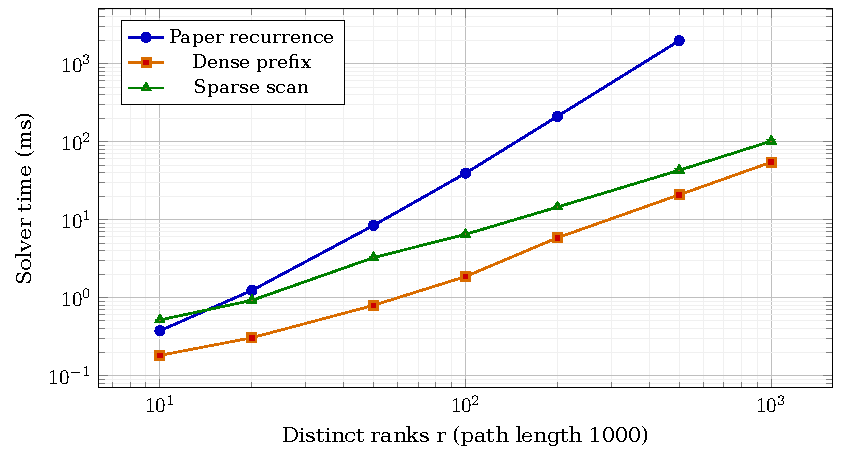
\includegraphics[width=0.94\textwidth]{../results/figures/forest-scaling.pdf}
\caption{Forest dài 1000 cạnh: median và IQR theo compressed $r$. Các điểm timeout của baseline không được vẽ thành giá trị hữu hạn.}
\label{fig:forest-repeated}
\end{figure}

Trong grid thưa ban đầu, một nhãn trồng chung trên mỗi cạnh cho đáp án không rỗng, nhưng tại cardinality một thì $r$ cũng nén còn một. Follow-up density control khắc phục: thêm một cạnh lá ngoài đường $s$--$z$ mang tất cả 1000 hạng. Nhờ vậy $r=1000$ cố định, đường có 1000 cạnh và thay đổi riêng cardinality nhãn trên đường. Cạnh lá không tạo thêm đường đi đơn giữa hai terminal.

\begin{table}[htbp]
\centering
\small
\setlength{\tabcolsep}{4pt}
\caption{Kiểm soát mật độ: đường dài 1000 cạnh, compressed rank cố định 1000.}
\label{tab:density-control}
\begin{tabular}{lrrrrr}
\toprule
Nhãn/cạnh $d$ & $r$ & Paper ms & Dense ms & Sparse ms & Dense/Sparse \\
\midrule
1 & 1000 & 6.94 & 3.33 & 0.228 & 14.6 \\
4 & 1000 & 10.9 & 3.38 & 0.338 & 10 \\
16 & 1000 & 28.9 & 3.69 & 0.905 & 4.08 \\
100 & 1000 & 189 & 6.98 & 6.64 & 1.05 \\
1000 & 1000 & T/O & 64.9 & 119 & 0.545 \\
\bottomrule
\end{tabular}
\end{table}

\begin{figure}[htbp]
\centering
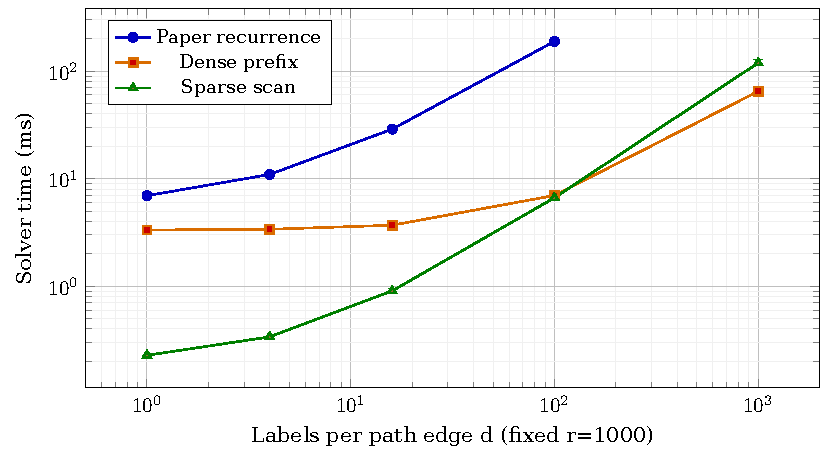
\includegraphics[width=0.94\textwidth]{../results/figures/density-control.pdf}
\caption{Giữ compressed $r=1000$ và chiều dài đường cố định, thay đổi số nhãn trên cạnh đường đi.}
\label{fig:density-control}
\end{figure}

H2 được đánh giá bằng phép đo kiểm soát này thay vì chỉ lấy graph có timestamp số lớn. Khi nhãn dày, mảng prefix có locality tốt hơn và có thể nhanh hơn sparse scan; khi nhãn ít, sparse solver tránh quét miền hạng trống. Vì các solver cùng kiểm tra cấu trúc và tra map, chi phí cố định giới hạn tỷ số tại cell nhỏ.

\FloatBarrier
\section{TTSP: ma trận so với sự kiện}

Mọi cell trong grid $k\in\{1,2,4,8,16,32,64,128,256\}$ và $r\in\{2,4,8,16,32\}$ đều được so đáp án với $2^k\binom{r+2k-1}{2k}$ bằng số nguyên Python; cả hai solver hoàn thành bảy lần đo trên toàn bộ 45 cell. Các cell strict dùng $2^k\binom{r}{2k}$. Đây là kiểm tra oracle trên toàn grid, không chỉ các trường hợp brute force nhỏ.

\begin{table}[htbp]
\centering
\small
\setlength{\tabcolsep}{4pt}
\caption{TTSP: median thời gian và maximum peak RSS qua các lần đo; skip là giới hạn ngân sách.}
\label{tab:ttsp-repeated}
\begin{tabular}{lrrrrrr}
\toprule
$k$ & $r$ thật & Matrix ms & Events ms & M/E & RSS M/E MiB & Bit \\
\midrule
1 & 32 & 0.736 & 0.0249 & 29.6 & 4.12/3.85 & 11 \\
16 & 32 & 18.5 & 0.393 & 47.2 & 9.2/4.09 & 76 \\
64 & 32 & 79 & 1.6 & 49.2 & 25.4/4.8 & 174 \\
256 & 32 & 365 & 7.53 & 48.4 & 92.6/8.01 & 424 \\
32 & 128 & 1.71e+03 & 2.2 & 776 & 167/5.65 & 204 \\
1024 & 7082 & skip & 14.8 & -- & --/7.14 & 1029 \\
\bottomrule
\end{tabular}
\end{table}


Tại $k=256,r=32$, graph có 1024 cạnh tĩnh, 32768 cạnh thời gian và đáp án 424 bit. Median ma trận là \TTSPMatrixTime{} ms; sự kiện là \TTSPEventTime{} ms, tỷ số \TTSPSpeedup{} lần. Maximum peak RSS qua các mẫu lần lượt \TTSPMatrixRSS{} và \TTSPEventRSS{} MiB. Telemetry quét sự kiện ghi đúng một phép cộng cho mỗi cạnh thời gian, phù hợp với cận số học trong \cref{thm:ttsp-events}.

\begin{figure}[htbp]
\centering
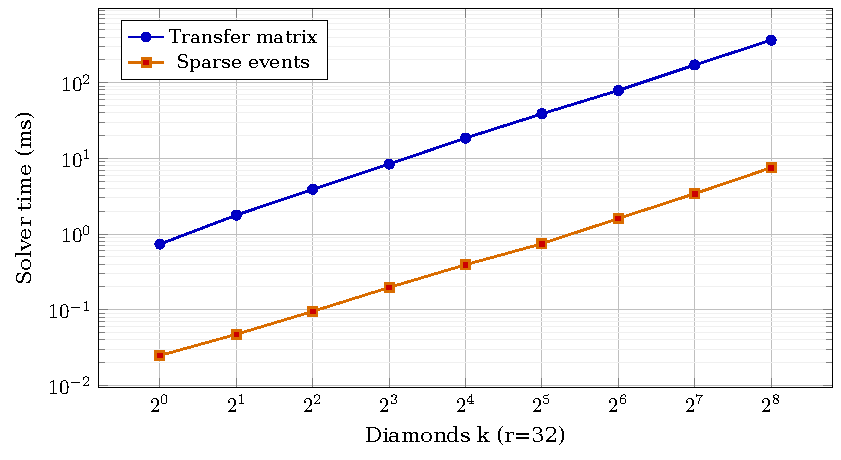
\includegraphics[width=0.94\textwidth]{../results/figures/ttsp-scaling.pdf}
\caption{TTSP tại $r=32$, median và IQR. Chi phí đọc/validate SP vẫn nằm trong thời gian solver.}
\label{fig:ttsp-events}
\end{figure}

Các graph thưa đến 1024 diamond dùng miền timestamp nominal 10000 và bốn nhãn/cạnh; bảng báo $r$ thực sự sau compression. Oracle vector SP bằng Python xác nhận count dù không thể liệt kê $2^{1024}$ tuyến. Ma trận vượt rank cap được ghi skip, không gán speedup hữu hạn cho một phép đo chưa chạy. Lõi sự kiện có cùng cơ sở đúng cho strict, nhưng benchmark strict là một tập riêng nhỏ hơn benchmark non-strict.

\FloatBarrier
\section{Treewidth: cận mới và miền thực dụng}

Trên 24 partial 2-tree cùng hoàn thành, trung bình nhân speedup DP mới so với DP cũ là \DPGeoSpeedup{} lần. Figure cố định $r=4$ và graph replicate 0 theo $n$; các seed khác nhau được nhận dạng trong raw CSV, nên không nhầm đây là cùng một graph được tăng dần đỉnh.

\begin{figure}[htbp]
\centering
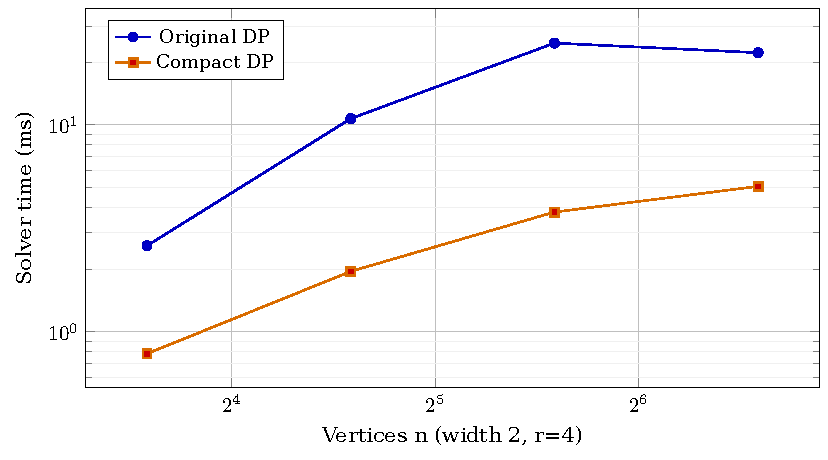
\includegraphics[width=0.94\textwidth]{../results/figures/partial2-scaling.pdf}
\caption{Partial 2-tree với terminal tùy ý: DP ban đầu và DP compact.}
\label{fig:partial2-scaling}
\end{figure}

\begin{table}[htbp]
\centering
\small
\setlength{\tabcolsep}{4pt}
\caption{Độ nhạy theo width tại n=12, r=8; mỗi width dùng một seed cố định.}
\label{tab:width-sensitivity}
\begin{tabular}{lrrrr}
\toprule
$w$ & Brute ms & DP cũ ms & DP mới ms & Trạng thái mới \\
\midrule
1 & 0.00117 & 0.429 & 0.171 & 272 \\
2 & 0.0312 & 17.5 & 3.07 & 4.83e+03 \\
3 & 1.49 & 272 & 15 & 1.8e+04 \\
4 & 12.7 & T/O & 381 & 4.32e+05 \\
\bottomrule
\end{tabular}
\end{table}

\begin{figure}[htbp]
\centering
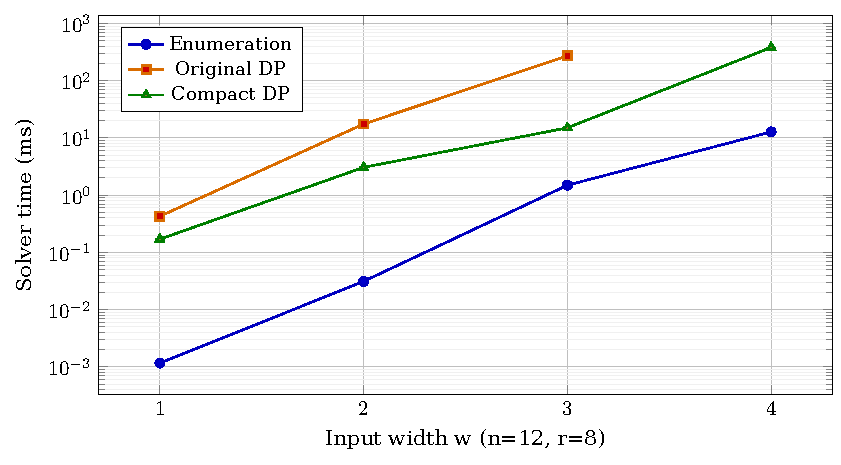
\includegraphics[width=0.94\textwidth]{../results/figures/width-scaling.pdf}
\caption{Độ nhạy với width tại $n=12,r=8$. Enumeration được đo và không bị loại khi thắng ở miền nhỏ.}
\label{fig:width-sensitivity}
\end{figure}

Ở $n=12$, enumeration có thể thắng DP vì chi phí tổ chức trạng thái lớn hơn lượng đường phải liệt kê. Khi width tăng, số trạng thái và chi phí join tăng mạnh dù số đỉnh không đổi. Điều này phù hợp với XP: cận đa thức khi width cố định không đồng nghĩa mọi width đều thực dụng. Bảng timeout thể hiện giới hạn đo được thay vì dùng chúng để khẳng định FPT.

\begin{table}[htbp]
\centering
\small
\setlength{\tabcolsep}{4pt}
\caption{Ablation trên ba partial 2-tree: GM của median thời gian; median telemetry theo instance.}
\label{tab:ablation}
\begin{tabular}{lrrrr}
\toprule
Cấu hình & Median-GM ms & States & Peak live & Join thử/có thể \\
\midrule
DP cũ & 32.4 & 18\,785 & 18\,785 & 100\% \\
Đầy đủ & 5.46 & 6\,801 & 854 & 40.1\% \\
Bỏ compact & 11.8 & 11\,324 & 2\,197 & 37.5\% \\
Bỏ prune và compact & 24.9 & 18\,785 & 4\,957 & 34.6\% \\
Bỏ index join & 6.49 & 6\,801 & 854 & 100\% \\
Giữ bảng con & 5.73 & 6\,801 & 6\,801 & 40.1\% \\
\bottomrule
\end{tabular}
\end{table}


Tỷ số trung bình nhân giữa baseline và bản đầy đủ trên ba instance ablation là \AblationCombinedSpeedup{} lần. \code{no-compact} giữ pruning nhưng lưu timestamp terminal; \code{no-prune} cũng phải tắt compaction vì quotient dựa trên ràng buộc terminal. Muốn tách riêng pruning, so \code{no-prune} với \code{no-compact}; muốn tách compaction, so \code{no-compact} với bản đầy đủ. \code{no-index} và \code{no-release} lần lượt đổi một yếu tố. Peak live states đo vòng đời bảng, còn RSS đo toàn address space, nên hai đại lượng không được đồng nhất.

\FloatBarrier
\section{Enumeration crossover và ladder hàm mũ}

\begin{table}[htbp]
\centering
\small
\setlength{\tabcolsep}{4pt}
\caption{Enumeration crossover tại width 2, r=4; các seed khác nhau được báo cáo đầy đủ.}
\label{tab:enumeration-crossover}
\begin{tabular}{lrr}
\toprule
$n$ & Enumeration ms & Treewidth ms \\
\midrule
12 & 0.0242 & 0.751 \\
24 & 1.07 & 2.03 \\
48 & 1.23 & 4.01 \\
96 & 98.7 & 5.09 \\
\bottomrule
\end{tabular}
\end{table}


Không tuyên bố DP luôn nhanh hơn enumeration: ở các graph ngẫu nhiên nhỏ, baseline đơn giản có thể thắng. Crossover còn phụ thuộc query, nhãn và topology. Để tách tác động số tuyến, ladder hai hàng tạo một họ width hai với oracle độc lập và số tuyến tăng hàm mũ.

\begin{proposition}[Oracle ladder]
Ladder $c$ cột, nguồn top-left và đích bottom-right, có $2^{c-1}$ đường đi tĩnh đơn. Nếu mỗi cạnh hoạt động ở mọi hạng $1..r$, số non-strict temporal paths là
\[
 \sum_{\substack{1\le q\le c\\q\ \mathrm{lẻ}}}
 \binom cq\binom{r+c+q-2}{c-1+q}.
\]
Với strict, thay thừa số thứ hai bằng $\binom r{c-1+q}$.
\end{proposition}

\begin{proof}
Mỗi cut giữa hai cột có đúng hai cạnh ngang. Đường đơn nối nguồn bên trái với đích bên phải phải vượt cut số lần lẻ và dùng mỗi cạnh tối đa một lần; vì thế vượt đúng một lần, theo hướng trái sang phải. Đường chọn một tập $q$ rung tại các cột; cần $q$ lẻ để đổi từ hàng trên sang hàng dưới. Mỗi tập rung lẻ xác định duy nhất một đường đơn dài $c-1+q$. Có $\binom cq$ tuyến tương ứng; áp dụng oracle nhãn cho từng độ dài. Tổng số tập con lẻ là $2^{c-1}$.
\end{proof}

Ladder từ ba cột không phải cactus; các cạnh có thể thuộc nhiều chu trình. Hai đường đơn của cùng truy vấn có thể dùng một rung theo hai hướng trái ngược, nên không áp dụng định hướng TTSP cực--cực sẵn có. Đây là stress case cho thuật toán SP với đầu cuối tùy ý, không chỉ cho solver cactus.

\begin{table}[htbp]
\centering
\small
\setlength{\tabcolsep}{4pt}
\caption{Ladder width hai với r=4 và truy vấn top-left/bottom-right; oracle đóng cho mọi cell.}
\label{tab:ladder}
\begin{tabular}{lrrrr}
\toprule
Cột $c$ & Tuyến tĩnh & Brute ms & DP cũ ms & DP mới ms \\
\midrule
4 & $2^{3}$ & 0.00737 & 1.3 & 0.303 \\
8 & $2^{7}$ & 0.25 & 3.73 & 0.876 \\
12 & $2^{11}$ & 6.25 & 5.76 & 1.47 \\
16 & $2^{15}$ & 138 & 9.07 & 2.04 \\
24 & $2^{23}$ & T/O & 14.2 & 3.16 \\
32 & $2^{31}$ & T/O & 19.4 & 4.66 \\
64 & $2^{63}$ & T/O & 40.6 & 9.38 \\
\bottomrule
\end{tabular}
\end{table}

\begin{figure}[htbp]
\centering
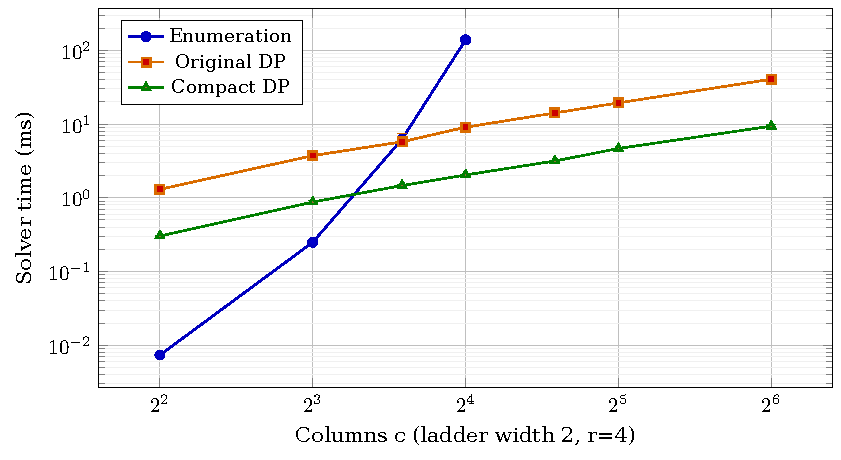
\includegraphics[width=0.94\textwidth]{../results/figures/ladder-scaling.pdf}
\caption{Ladder width hai tại $r=4$. Median/IQR của enumeration và hai phiên bản DP; cell timeout được giữ trong bảng.}
\label{fig:ladder-scaling}
\end{figure}

Ladder 64 cột có $2^{63}$ tuyến tĩnh. DP trả count chính xác so với công thức, trong khi enumeration vượt timeout. Điều này kiểm chứng khả năng nén nghiệm mà các instance rất nhỏ dùng làm oracle không thể thể hiện.

\FloatBarrier
\section{Cactus với truy vấn nội bộ}

Chọn hai đỉnh giữa ở diamond đầu và cuối của chuỗi $k\ge2$ diamond. Mỗi block đầu/cuối có hai cung dài một hoặc ba; các block giữa đóng góp hai lựa chọn dài hai. Oracle là
\[
2^{k-2}\left[
 \binom{r+2k-3}{2k-2}+2\binom{r+2k-1}{2k}+\binom{r+2k+1}{2k+2}
\right].
\]
Query không trùng cực gốc của biểu thức ban đầu. Cactus solver tự xây route theo query, không nhận decomposition ngoài. Trung bình nhân speedup so với generic treewidth DP trên tám cell là \CactusGeoSpeedup{} lần; đây là so sánh nội bộ giữa hai thuật toán của khóa luận.

\begin{table}[htbp]
\centering
\small
\setlength{\tabcolsep}{4pt}
\caption{Cactus với đầu cuối nội bộ tùy ý; toàn bộ đáp án đối chiếu công thức độc lập.}
\label{tab:cactus-repeated}
\begin{tabular}{lrrr}
\toprule
$k$ & Cactus ms & Treewidth ms & DP/Cactus \\
\midrule
4 & 0.0208 & 2 & 96.1 \\
16 & 0.0989 & 11.8 & 119 \\
64 & 0.354 & 51.3 & 145 \\
256 & 1.53 & 218 & 143 \\
\bottomrule
\end{tabular}
\end{table}

\begin{figure}[htbp]
\centering
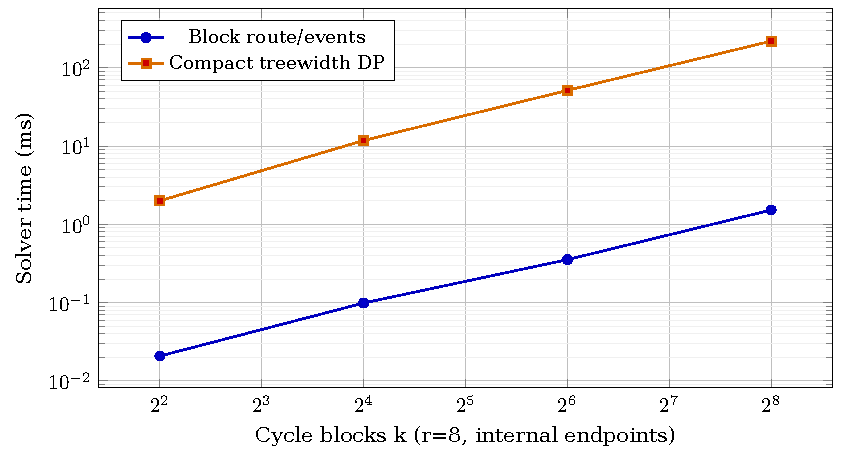
\includegraphics[width=0.94\textwidth]{../results/figures/cactus-scaling.pdf}
\caption{Cactus có đầu cuối nội bộ: block route/sự kiện và DP treewidth tổng quát.}
\label{fig:cactus-scaling}
\end{figure}

\FloatBarrier
\section{Censoring và giới hạn}

\begin{table}[htbp]
\centering
\small
\setlength{\tabcolsep}{4pt}
\caption{Mọi solver/cell không hoàn thành; không bị loại khỏi báo cáo.}
\label{tab:censored}
\begin{tabular}{llll}
\toprule
Họ & Instance & Solver & Trạng thái \\
\midrule
forest\_dense & L500-r1000 & forest-paper & timeout \\
forest\_dense & L1000-r1000 & forest-paper & timeout \\
forest\_sparse & L1000-r1000-d1000 & forest-paper & timeout \\
forest\_density\_control & L1000-r1000-d1000 & forest-paper & timeout \\
ttsp\_extra & k64-r128-strict0 & ttsp-transfer & timeout \\
ttsp\_sparse & k64-r1000-d4 & ttsp-transfer & skipped\_budget \\
ttsp\_sparse & k256-r10000-d4 & ttsp-transfer & skipped\_budget \\
ttsp\_sparse & k1024-r10000-d4 & ttsp-transfer & skipped\_budget \\
width & w4-n12-r8 & tw-dp-baseline & timeout \\
ladder & c24-r2 & brute & timeout \\
ladder & c24-r4 & brute & timeout \\
ladder & c24-r8 & brute & timeout \\
ladder & c32-r2 & brute & timeout \\
ladder & c32-r4 & brute & timeout \\
ladder & c32-r8 & brute & timeout \\
ladder & c64-r2 & brute & timeout \\
ladder & c64-r4 & brute & timeout \\
ladder & c64-r8 & brute & timeout \\
\bottomrule
\end{tabular}
\end{table}


T/O là subprocess không kết thúc trong ba giây; skip là quyết định ngân sách trước khi chạy. Không thay timeout bằng đúng ba giây để tính median, không loại chúng khỏi bảng phạm vi, và không lấy ratio của hai loại timing khác nhau. CSV/summary đầy đủ là nguồn số liệu chính; các bảng trong chương chỉ chọn cell đại diện theo kích thước đã mô tả.

\paragraph{Nội tại.} BigInt tự cài có rủi ro, được kiểm tra bằng số nguyên Python, oracle đóng và sanitizer. Bảy mẫu và pinning giảm nhiễu nhưng không khóa tần số hay tạo máy benchmark riêng. RSS không đo chính xác heap được dùng cho DP. Lõi $\bigO(M)$ theo số phép cộng vẫn có chi phí tăng với số bit.

\paragraph{Ngoại tại.} Dữ liệu chính là synthetic theo theorem và Graph Atlas cho correctness. Không có mạng thời gian thực trong chiến dịch này; graph thực có width cao không tự thuộc miền thuật toán. Vì vậy không suy rộng tốc độ SP sang mọi mạng xã hội/giao thông.

\paragraph{Kết luận.} Audit lớn không chứng minh đúng thay cho chứng minh; chưa vét cạn $n=5,r=2$. Tham số và seed được ghi rõ, nhưng vài graph mỗi cell không đại diện cho mọi phân phối. Geometric mean chỉ dùng cell cùng hoàn thành và không diễn tả riêng tỷ lệ timeout; hai chỉ số được báo song song.

\paragraph{Tính mới.} Rà soát cập nhật đọc thêm các nguồn 2025--2026, nhưng chưa có kết luận phản biện độc lập về ưu tiên công bố. Khóa luận đã đưa ra định lý, mã và bằng chứng kiểm tra; việc xác lập kết quả học thuật cuối cùng là bước thẩm định riêng.
